\documentclass{ieeeaccess}
\usepackage{cite}
\usepackage{amsmath,amssymb,amsfonts}
\usepackage{algorithmic}
\usepackage{algorithm}
\usepackage{graphicx}
\usepackage{textcomp}
\usepackage{caption}
\usepackage{subcaption}
\def\BibTeX{{\rm B\kern-.05em{\sc i\kern-.025em b}\kern-.08em
    T\kern-.1667em\lower.7ex\hbox{E}\kern-.125emX}}
\begin{document}
\history{Date of publication xxxx 00, 0000, date of current version xxxx 00, 0000.}
\doi{10.1109/ACCESS.2017.DOI}

\title{Handling uncertain Predictions of Vascular Access Dysfunction in Chronic Hemodialysis Patients through Tree-Based Approaches}
\author{\uppercase{Zheng Lin Chen}\authorrefmark{1},
\uppercase{Second B. Author\authorrefmark{2}, and Third C. Author,
Jr}.\authorrefmark{3},
\IEEEmembership{Member, IEEE}}
\address[1]{College of Artificial Intelligence, National Yang Ming Chiao Tung University, Taiwan (email: zhenglin.ai11@nycu.edu.tw)}
\address[2]{Department of Physics, Colorado State University, Fort Collins, 
CO 80523 USA (e-mail: author@lamar.colostate.edu)}
\address[3]{Electrical Engineering Department, University of Colorado, Boulder, CO 
80309 USA}
\tfootnote{This paragraph of the first footnote will contain support 
information, including sponsor and financial support acknowledgment. For 
example, ``This work was supported in part by the U.S. Department of 
Commerce under Grant BS123456.''}

\markboth
{Author \headeretal: Preparation of Papers for IEEE TRANSACTIONS and JOURNALS}
{Author \headeretal: Preparation of Papers for IEEE TRANSACTIONS and JOURNALS}

\corresp{Corresponding author: First A. Author (e-mail: author@ boulder.nist.gov).}

\begin{abstract}
Vascular access dysfunction is a prevalent and critical complication among hemodialysis patients, particularly in Taiwan, which has the highest proportion of dialysis patients globally. Early diagnosis and effective management are vital to improving patient outcomes. However, traditional diagnostic approaches, such as routine surveillance and fixed blood flow thresholds, often fail to reliably identify patients requiring timely surgical intervention. To address these challenges, this study proposes a trustworthy AI system utilizing an uncertain-aware, tree-based machine learning framework to enhance the assessment of vascular access dysfunction.

The proposed framework incorporates tree-based models, including Decision Trees, Random Forests, and XGBoost, alongside advanced uncertainty quantification techniques. By employing a multipass perturbation strategy to simulate sample variability, the framework effectively identifies uncertain cases, ensuring robust and interpretable predictions. Furthermore, this study introduces an extended confusion matrix and novel uncertainty metrics to evaluate model performance comprehensively. The framework's design emphasizes toward zero-leakage rate AI by minimizing overconfident misclassifications, thereby improving the reliability of clinical decision-making and reducing unnecessary interventions. The system has been validated using real-world hospital datasets, demonstrating its deployable AI potential with superior predictive accuracy, sensitivity, and robustness compared to traditional methods, such as KDOQI guidelines.
\end{abstract}

\begin{keywords}
Deployable AI, Uncertainty Quantification, Machine Learning, Toward Zero Leakage Rate AI, Tree-Based Models, Trustworthy AI System, Vascular Access Dysfunction
\end{keywords}

\titlepgskip=-15pt

\maketitle

\section{Introduction}
\label{sec:introduction}
\PARstart{H}{emodialysis} is a vital treatment for patients with end-stage renal disease (ESRD), and vascular access dysfunction is a major complication that directly impacts treatment efficacy and patient survival. Taiwan, which has the highest prevalence of dialysis patients globally, faces significant challenges in the early detection and management of vascular access dysfunction. Traditional diagnostic methods, such as physical examinations and fixed flow rate thresholds from the KDOQI guidelines, often fail to account for patient-specific variability, leading to missed or delayed interventions.

Recent advances in machine learning, particularly tree-based models like Decision Trees, Random Forests, and XGBoost, offer opportunities to enhance diagnostic precision through structured data classification. These models, when combined with uncertainty quantification techniques, can provide robust and interpretable predictions, addressing the limitations of traditional methods.

\subsection{Motivation}
Despite established guidelines, significant challenges remain in predicting vascular access dysfunction with high confidence. Patient variability, the limitations of fixed thresholds, and the inability to manage ambiguous cases necessitate a new approach. Current studies often prioritize predictive accuracy while neglecting interpretability and the management of uncertainty, creating a critical gap in clinical applicability.

\subsection{Goal}
This study aims to develop an uncertain-aware, tree-based machine learning framework to improve the prediction and management of vascular access dysfunction. The proposed framework integrates:
\begin{itemize}
    \item uncertainty quantification to address ambiguous cases.
    \item Machine learning models that balance accuracy and interpretability.
    \item Clinical guidelines (e.g., KDOQI) with data-driven methodologies to enhance diagnostic adaptability.
\end{itemize}
By addressing these challenges, this research seeks to improve the timeliness and reliability of interventions, ultimately benefiting patient outcomes and healthcare efficiency.

\section{Related Works}

\subsection{KDOQI Guidelines}
The 2006 KDOQI guidelines~\cite{KDOQI} provide a comprehensive framework for managing vascular access in hemodialysis patients, emphasizing flow rate thresholds: <500 mL/min for arteriovenous fistulas (AVFs) and <600 mL/min for grafts (AVGs). While effective, these static thresholds often fail to address patient-specific variability, leading to missed interventions. Recent advancements in AI, such as machine learning-enhanced clinical decision support systems~\cite{Balch_2024}, highlight the potential to augment these guidelines with adaptive and precise diagnostic capabilities.

\subsection{Physical Examination}
Routine vascular access surveillance combined with physical examinations has demonstrated high predictive accuracy for stenosis detection, particularly for AVFs~\cite{Wu}. Absolute flow thresholds (<500 mL/min for AVFs and <600 mL/min for AVGs) outperform relative thresholds in clinical decision-making. Despite its success, challenges persist in AVG monitoring due to structural differences, underscoring the need for supplementary diagnostic tools like duplex ultrasound and advanced machine learning approaches for enhanced prediction and timely intervention.

\subsection{Tree-Based Models}

%Tree-based machine learning models, including Decision Trees\cite{decision_tree}, Random Forests\cite{random_forest}, and XGBoost\cite{XGBoost}, are widely used for structured data analysis due to their interpretability and computational efficiency. While Decision Trees are simple but prone to overfitting, ensemble methods like Random Forests mitigate this by reducing variance through bagging. XGBoost leverages boosting techniques for improved accuracy and scalability~\cite{Comparative_XGBoost}, making it a preferred choice in clinical applications. Advanced models like LightGBM and CatBoost further enhance performance through selective sampling and categorical feature handling~\cite{LightGBM, CatBoost}, ensuring adaptability across diverse datasets.

Tree-based models, including Decision Trees~\cite{decision_tree}, Random Forests~\cite{random_forest}, and XGBoost~\cite{XGBoost}, are widely used for structured data analysis due to their interpretability, computational efficiency, and ability to handle heterogeneous data. These models excel on tabular datasets, which often feature a mix of numerical and categorical variables, irregular patterns, and skewed distributions. Tree-based methods efficiently capture these characteristics through piecewise constant functions, requiring minimal preprocessing and feature engineering, unlike neural networks, which demand extensive regularization and transformation to handle similar datasets effectively.

Research highlights the superior performance of tree-based models in structured data scenarios. Random Forests mitigate overfitting through variance reduction via bagging, while XGBoost leverages boosting techniques for enhanced accuracy and scalability~\cite{Comparative_XGBoost}. Advanced models like LightGBM and CatBoost further improve efficiency through selective sampling and categorical feature handling~\cite{LightGBM, CatBoost}. Studies by Grinsztajn et al.\cite{tree_based_model} and McElfresh and Khandagale\cite{Outperform_Boosted_Trees} demonstrate that Gradient Boosted Decision Trees (GBDTs) outperform neural networks on medium-sized tabular datasets, where the latter often fail to generalize. Similarly, Ye et al.~\cite{Closer_Look} find that while deep learning has made strides, tree-based models remain competitive, particularly in scenarios with limited data or computational resources. These strengths make tree-based models a robust, practical choice for structured data, where their adaptability and efficiency surpass neural networks.

\subsection{Ensemble Learning}
Ensemble methods, such as bagging and boosting, enhance robustness by combining multiple classifiers~\cite{9893798}. This study employs a soft voting ensemble of Decision Trees, Random Forests, and XGBoost, integrating model predictions probabilistically to improve accuracy and balance. Tree-based ensembles are particularly effective for structured data, addressing imbalanced datasets and hierarchical relationships, while maintaining superior interpretability compared to neural networks.

\subsection{Uncertainty Handling and Interpretability}
Uncertainty quantification addresses ambiguous cases by categorizing predictions into determinate and uncertain groups~\cite{Uncertainty_Quantification}. Techniques like multipass perturbation and rejection strategies~\cite{electronics11030396} improve prediction reliability and enable cautious decision-making in high-stakes clinical scenarios. Additionally, interpretability methods such as local perturbation analysis provide insights into model behavior and feature contributions~\cite{perturbations}, enhancing transparency and trustworthiness. These advancements are integrated into this study’s framework, ensuring robust and explainable predictions tailored for clinical applications.

\section{Method}
This chapter outlines the methods used to enhance the predictive accuracy and robustness of the proposed uncertainty-aware classification framework. The methodology includes three core components: data preprocessing and model training, multipass uncertainty estimation, and uncertain-aware classification.

\subsection{Model Architecture}
The proposed framework utilizes tree-based models—Decision Tree, Random Forest, and XGBoost—with a weighted soft voting strategy to combine their predictions. These models were trained using K-fold cross-validation to ensure reliable performance.

Key preprocessing steps included removing redundancies, feature creation, and data alignment. To address class imbalance, the \texttt{scale\_pos\_weight}
parameter was tuned in XGBoost. This architecture provides a robust foundation for integrating uncertainty quantification.

\subsection{Multipass Uncertainty Estimation}
To quantify prediction uncertainty, a multipass estimation method was developed. This involves generating perturbed versions of each input sample by adding Gaussian noise, then passing these perturbed samples through the ensemble model to compute probability means ($p_{u}$) and variances ($p_{\sigma^2}$).

Steps:
\begin{enumerate}
    \item \textbf{Perturbation}: Gaussian noise ($\epsilon \sim N(\mu, \sigma^2)$) is added to simulate variability.
    \item \textbf{Prediction}: Perturbed samples are processed by the soft voting ensemble to predict probabilities for "True" and "False."
    \item \textbf{Aggregation}: Means and variances of probabilities across all perturbed samples are calculated.
\end{enumerate}

\subsection{Uncertain-Aware Classification}
Based on the results of multipass estimation, samples are categorized into "True," "False," or "Uncertain" classes using entropy and confidence thresholds.

Steps:
\begin{enumerate}
    \item \textbf{Entropy Calculation}: Compute the entropy $H(y_p,\mu)$ of the probability distribution. Samples with entropy exceeding a predefined threshold ($\theta_{u}$) are classified as "Uncertain."
    \begin{equation}
    H(y_p,\mu) = -(p_{T,\mu}\log p_{T,\mu}+p_{F,\mu}\log p_{F,\mu})
    \end{equation}
    \item \textbf{Confidence Evaluation}: For samples with low entropy, their mean probabilities ($p_{u}$) and variances ($p_{\sigma^2}$) are used to classify them as "True" or "False," considering variability to avoid overconfident misclassification.
\end{enumerate}

Classification Rules:
\begin{itemize}
    \item A sample is "True" if:
    \begin{equation}
    p_{T,\mu} > p_{F,\mu} \textbf{ and } p_{T,\mu} - \sqrt{p_{T,\sigma^2}} > p_{F,\mu} + \sqrt{p_{F,\sigma^2}}
    \end{equation}
    \item A sample is "False" if:
    \begin{equation}
    p_{F,\mu} > p_{T,\mu} \textbf{ and } p_{F,\mu} - \sqrt{p_{F,\sigma^2}} > p_{T,\mu} + \sqrt{p_{T,\sigma^2}}
    \end{equation}
\end{itemize}
Samples not meeting these conditions are classified as "Uncertain."

\subsection{Algorithm Overview}
Algorithm 1: Multipass Uncertainty Estimation generates probability distributions for perturbed samples, quantifying prediction variability. Algorithm 2: Uncertain-Aware Classification uses entropy and confidence thresholds to make final classifications, ensuring robust decisions for ambiguous cases.

These methods address the limitations of fixed-threshold diagnostic systems by providing adaptive and cautious predictions, particularly for borderline cases, enhancing utility in clinical settings.


\begin{algorithm}[H]
\caption{Multipass Uncertainty Estimation}
\label{alg:Training}
\begin{algorithmic}[1]
\renewcommand{\algorithmicrequire}{\textbf{Input:}}
\renewcommand{\algorithmicensure}{\textbf{Output:}}
\REQUIRE $\hat{x}$ (Input sample), $\mu$ (Noise mean), $\sigma^2$ (Noise variance), $W=[w_1, w_2, w_3]$ (Weights of estimators), $n$ (Number of passes),
$Estimators=[\text{Decision Tree, Random Forest, XGBoost}]$
\ENSURE $p_{\mu}$ (Mean of probabilities), $p_{\sigma^2}$ (Variance of probabilities)

\STATE \textit{Initialize:} $\hat{P} \gets [ ]$
\FOR {$i = 1$ to $n$}
    \STATE Sample $\epsilon_i \sim N(\mu, \sigma^2)$
    \STATE $\hat{x_i} \gets \hat{x} + \epsilon_i$
    \STATE $P_{y_i} \gets [ ]$
    \FOR {each $clf$ in $Estimators$}
        \STATE $v_{clf} \gets \text{VotingClassifier}(clf, \text{voting} = \text{'soft'})$
        \STATE $p_{y_{i}, clf} \gets v_{clf}.\text{PredictProb}(\hat{x_i})$ \hfill $\triangleright$ $p = [p_T, p_F]$
        \STATE Append $p_{y_{i}, clf}$ to $P_{y_i}$
    \ENDFOR
    \STATE $\hat{p_i} \gets \text{average}(P_{y_i}, W)$
    \STATE Append $\hat{p_i}$ to $\hat{P}$
\ENDFOR
\STATE $p_{\mu} \gets \text{mean}(\hat{P})$ \hfill $\triangleright$ $p_{\mu} = [p_{T,\mu}, p_{F,\mu}]$
\STATE $p_{\sigma^2} \gets \text{variance}(\hat{P})$ \hfill $\triangleright$ $p_{\sigma^2} = [p_{T,\sigma^2}, p_{F,\sigma^2}]$
\RETURN $p_{\mu}, p_{\sigma^2}$
\end{algorithmic}
\end{algorithm}

\begin{algorithm}[H]
\caption{Uncertain-Aware Data Classification}
\label{alg: UncertainClassification}
\begin{algorithmic}[1]
\renewcommand{\algorithmicrequire}{\textbf{Input:}}
\renewcommand{\algorithmicensure}{\textbf{Output:}}
\REQUIRE $p_{\mu} = [p_{T,\mu}, p_{F,\mu}]$ (Mean of probabilities)\\
\hspace{1.2em} $p_{\sigma^2} = [p_{T,\sigma^2}, p_{F,\sigma^2}]$ (Variance of probabilities)\\
\hspace{1.2em} $\theta_{\mu}$ (Uncertainty threshold)
\ENSURE "True", "False" or "Uncertain"

\STATE Compute entropy: $H(y_p,\mu) \gets -(p_{T,\mu}\log p_{T,\mu} + p_{F,\mu}\log p_{F,\mu})$
\IF {$H(y_p,\mu) > \theta_{\mu}$}
    \RETURN "Uncertain"
\ELSE
    \IF {$p_{T,\mu} > p_{F,\mu}$ \textbf{and} $p_{T,\mu} - \sqrt{p_{T,\sigma^2}} > p_{F,\mu} + \sqrt{p_{F,\sigma^2}}$}
        \RETURN "True"
    \ELSIF {$p_{F,\mu} > p_{T,\mu}$ \textbf{and} $p_{F,\mu} - \sqrt{p_{F,\sigma^2}} > p_{T,\mu} + \sqrt{p_{T,\sigma^2}}$}
        \RETURN "False"
    \ELSE
        \RETURN "Uncertain"
    \ENDIF
\ENDIF
\end{algorithmic}
\end{algorithm}

\section{Experiments and Results}
\subsection{Dataset Description}
This study uses a dataset from a hospital, comprising 5,860 records from 412 patients undergoing routine clinical monitoring. The data is divided into Arteriovenous Fistula (AVF) and Arteriovenous Graft (AVG) subsets, representing native and synthetic vascular access types, respectively. Each record includes constant clinical features, such as age, gender, and comorbidities, and dynamic procedural features like access site and QA values. The output data indicates whether a patient underwent Percutaneous Transluminal Angioplasty (PTA).

\subsection{Feature Engineering}
To align data temporally, records preceding surgery were adjusted to represent the surgical day, ensuring the features reflected the patient’s clinical status before intervention. New features, such as previous QA values, recent surgical indicators, and the slope of QA changes over time, were created to capture trends in vascular access performance. Inspired by KDOQI guidelines, these features provided clinically relevant metrics for predicting outcomes.

\subsection{Evaluation Metrics}
As shown in Figure \ref{fig:enter-ECM}, the extended confusion matrix includes six categories: True Positive (TP), False Negative (FN), False Positive (FP), True Negative (TN), Uncertain Positive (UP), and uncertain Negative (UN). This extension allows for a more granular assessment of prediction Uncertainty and misclassification risks, which are critical in clinical decision-making. By incorporating the IP and IN categories, the model can better quantify ambiguous predictions, minimizing overconfident errors and improving reliability. Metrics such as Positive Predictive Value (PPV), Negative Predictive Value (NPV), Error Rate, Leakage Rate, Overkill Rate, Uncertainty Rate, Imperfection Rate, Uncertain Recall, and Harmonic Score were employed to comprehensively evaluate model performance, manage uncertainty, and reduce misclassification risks.

\begin{figure}[H]
    \centering
    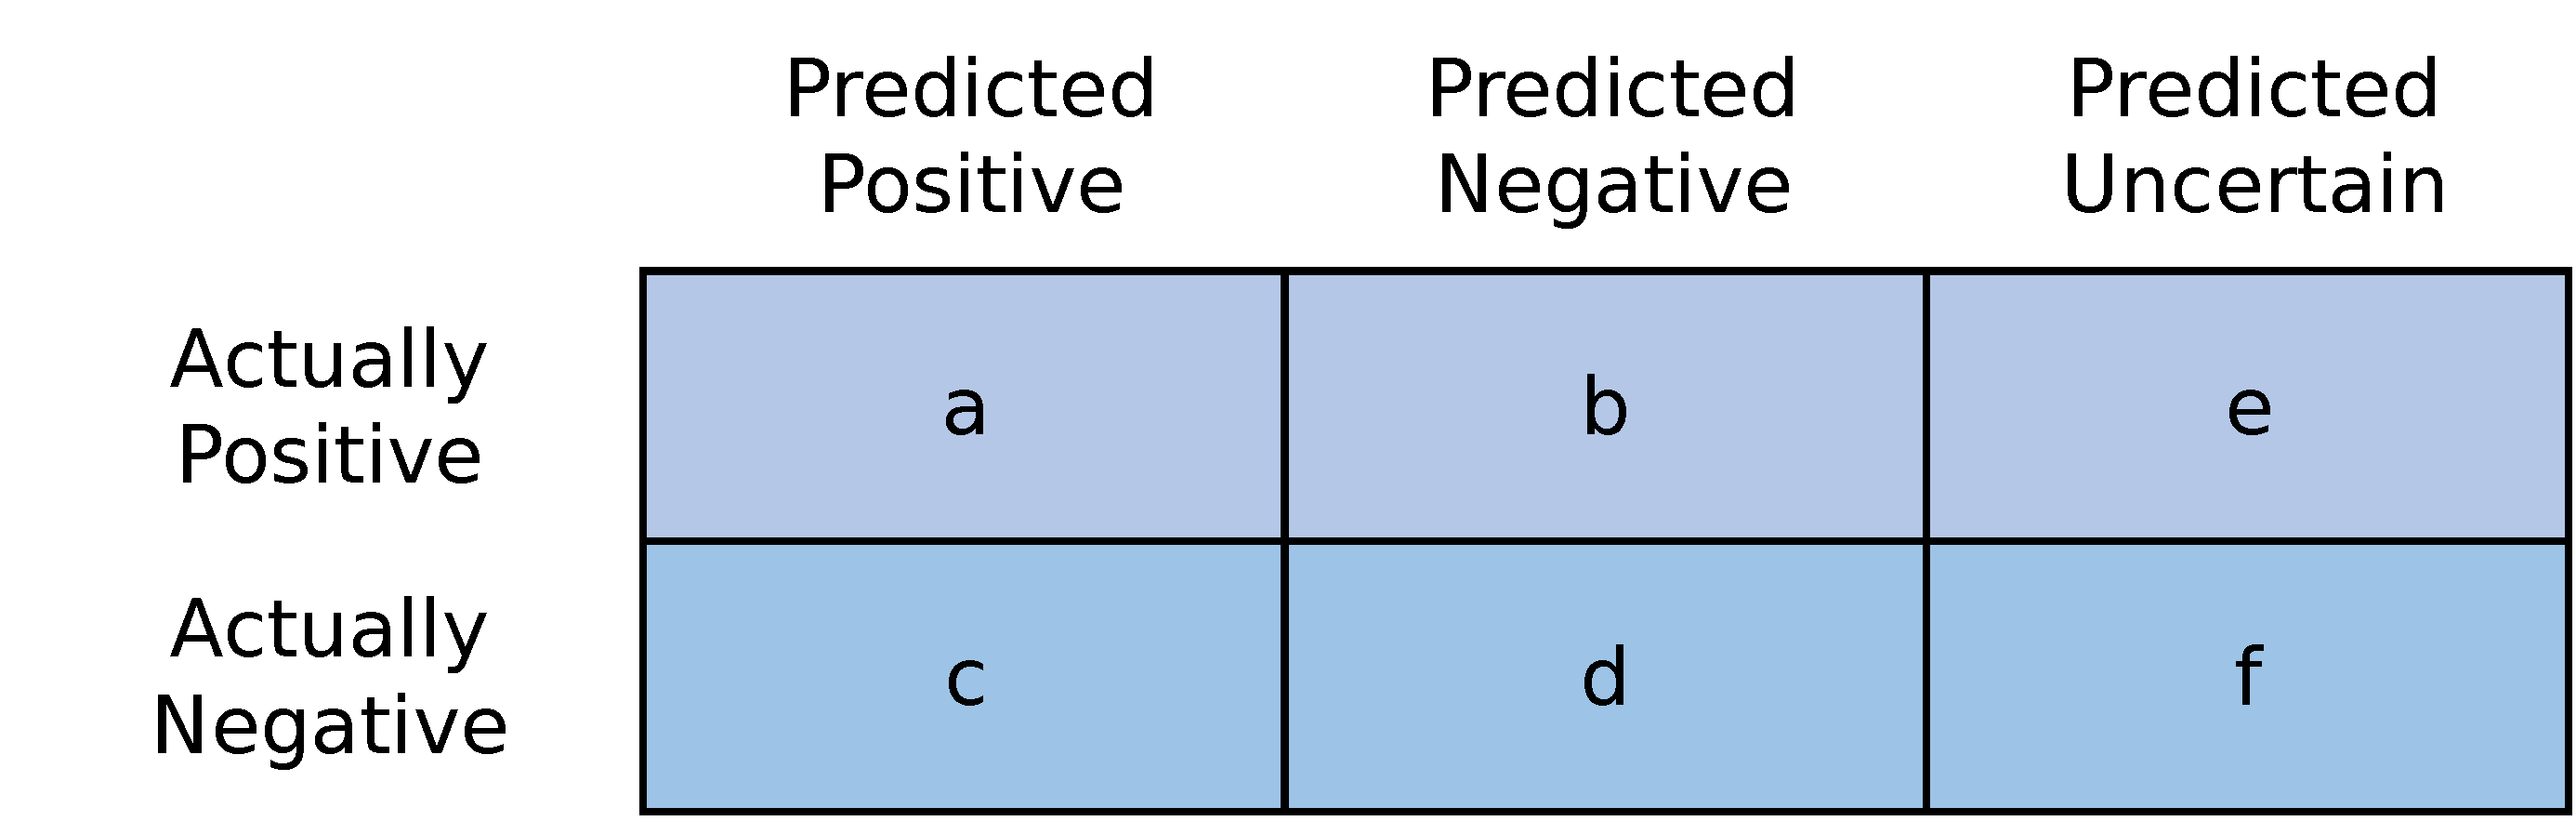
\includegraphics[width=1\linewidth]{new Extended confusion matrix.pdf}
    \caption{Extended confusion matrix. a: True Positive (TP), b: False Negative (FN), c: False Positive (FP), d: True Negative (TN), e: Uncertain Positive (UP), f: Uncertain Negative (UN)}
    \label{fig:enter-ECM}
\end{figure}

\begin{itemize}
  \item \textbf{Standard Metrics}: 
    \begin{equation}
        Accuracy = \frac{a + d}{a + b + c + d}
    \end{equation}
    \begin{equation}
        PPV = \frac{a}{a + c}
    \end{equation}
    \begin{equation}
        NPV = \frac{d}{b + d}
    \end{equation}
  \item \textbf{Uncertainty Metrics}: 
    \begin{equation}
        All = a + b + c + d + e + f
    \end{equation}
    \begin{equation}
        Error Rate = \frac{b + c}{All}
    \end{equation}
    \begin{equation}
        Leakage Rate = \frac{b}{All}
    \end{equation}
    \begin{equation}
        Overkill Rate = \frac{c}{All}
    \end{equation}
    \begin{equation}
        Uncertain Rate = \frac{e + f}{All}
    \end{equation}
    \begin{equation}
        Imperfection Rate = \frac{b + c + e + f}{All}
    \end{equation}
    \begin{equation}
        Uncertain Recall Rate = \frac{a + e}{a + b + e}
    \end{equation}
    \begin{equation}
        Harmonic Score = \frac{\frac{w_1'}{\exp\left(\frac{b}{All}\right)} + \frac{w_2'}{\exp\left(\frac{c}{All}\right)} + \frac{w_3'}{\exp\left(\frac{e + f}{All}\right)}}{3}
    \end{equation}
\end{itemize}

\subsection{Experiment Results}

The results of the evaluation metrics for both the Arteriovenous Fistula (AVF) and Arteriovenous Graft (AVG) datasets are summarized in Tables \ref{CombinedMetricsAVF} and \ref{CombinedMetricsAVG}, and visualized in Figures \ref{fig:AVF_ECM}, \ref{fig:AVF_combined-roc}, \ref{fig:AVG_ECM}, and \ref{fig:AVG_combined-roc}. Below is a detailed discussion of the findings:

\begin{itemize}
    \item \textbf{Arteriovenous Fistula (AVF) Dataset}\\
    As shown in Table \ref{CombinedMetricsAVF} and Figures \ref{fig:AVF_ECM} and \ref{fig:AVF_combined-roc}, the AVF dataset consisted of 4,991 cases, of which 10.9\% required Percutaneous Transluminal Angioplasty (PTA) interventions. The proposed uncertain-aware model achieved the highest accuracy of 91.3\%, outperforming the KDOQI guidelines (87.2\%) and the baseline model without uncertain classifications (89.5\%). This improvement was accompanied by a reduction in the Error Rate to 8.1\% and a Leakage Rate to 8.0\%. Additionally, the Area Under the Curve (AUC) increased significantly, from 0.62 for the KDOQI guidelines to 0.76 for the uncertain-aware model. These results emphasize the model's capability to handle ambiguous cases effectively, minimizing misclassification risks and enhancing prediction reliability.

    \item \textbf{Arteriovenous Graft (AVG) Dataset}\\
    As presented in Table \ref{CombinedMetricsAVG} and Figures \ref{fig:AVG_ECM} and \ref{fig:AVG_combined-roc}, the AVG dataset, comprising 869 cases with a higher PTA intervention rate of 25.1\%, posed unique challenges due to its smaller size and greater variability. The uncertain-aware model demonstrated superior performance, achieving an accuracy of 81.8\%, compared to 79.1\% for the baseline model. The Error Rate was reduced to 14.7\%, and the Leakage Rate was minimized to 12.8\%. Furthermore, the AUC increased from 0.62 (KDOQI) to 0.73, illustrating the model's robustness in adapting to datasets with higher variability and imbalance.

\end{itemize}

These results underscore the effectiveness of the proposed uncertain-aware framework in improving diagnostic performance for vascular access dysfunction. By incorporating uncertain classifications, the model not only enhances predictive accuracy but also reduces overconfident errors, ensuring more reliable and cautious decision-making in clinical settings.


\begin{table}[H]
\caption{AVF Dataset Evaluation Metrics for Baseline (KDOQI Guidelines), Our Method (Without Uncertain), and Our Method (With Uncertain)}
\label{CombinedMetricsAVF}
\setlength{\tabcolsep}{3pt}
\renewcommand{\arraystretch}{1.5}
\begin{tabular}{|p{80pt}|p{45pt}|p{45pt}|p{45pt}|}
\hline
Metric & Baseline (KDOQI Guidelines) & Our Method (Without Uncertain) & Our Method (With Uncertain) \\ 
\hline
Accuracy & 0.872 ± 0.001 & 0.895 ± 0.004 & \textbf{0.913 ± 0.001} \\ 
\hline
PPV (Positive Predictive Value) & 0.394 ± 0.011 & 0.589 ± 0.028 & \textbf{0.841 ± 0.043} \\ 
\hline
NPV (Negative Predictive Value) & 0.918 ± 0.003 & 0.904 ± 0.002 & 0.914 ± 0.001 \\ 
\hline
Error Rate & 0.129 ± 0.01 & 0.105 ± 0.004 & \textbf{0.081 ± 0.002} \\ 
\hline
Leakage Rate & 0.078 ± 0.012 & 0.093 ± 0.001 & \textbf{0.08 ± 0.002} \\ 
\hline
Overkill Rate & 0.051 ± 0.031 & 0.011 ± 0.003 & \textbf{0.002 ± 0.002} \\ 
\hline
Uncertain Rate & - & - & 0.073 ± 0.027 \\ 
\hline
Imperfection Rate & 0.129 ± 0.01 & 0.105 ± 0.004 & 0.154 ± 0.021 \\ 
\hline
Uncertain Recall & 0.261 ± 0.039 & 0.146 ± 0.014 & \textbf{0.292 ± 0.03} \\ 
\hline
Harmonic Score & 0.958 ± 0.002 & \textbf{0.967 ± 0.001} & 0.951 ± 0.008 \\ 
\hline
\end{tabular}
\end{table}

\begin{table}[H]
\caption{AVG Dataset Evaluation Metrics for Baseline (KDOQI Guidelines), Our Method (Without Uncertain), and Our Method (Uncertain)}
\label{CombinedMetricsAVG}
\setlength{\tabcolsep}{3pt}
\renewcommand{\arraystretch}{1.5}
\begin{tabular}{|p{80pt}|p{45pt}|p{45pt}|p{45pt}|}
\hline
Metric & Baseline (KDOQI Guidelines) & Our Method (Without Uncertain) & Our Method (With Uncertain) \\ 
\hline
Accuracy & 0.791 ± 0.018 & 0.765 ± 0.023 & \textbf{0.818 ± 0.019} \\ 
\hline
PPV (Positive Predictive Value) & 0.685 ± 0.044 & 0.695 ± 0.045 & \textbf{0.74 ± 0.137} \\ 
\hline
NPV (Negative Predictive Value) & 0.809 ± 0.026 & 0.788 ± 0.028 & \textbf{0.828 ± 0.031} \\ 
\hline
Error Rate & 0.208 ± 0.032 & 0.235 ± 0.023 & \textbf{0.147 ± 0.017} \\ 
\hline
Leakage Rate & 0.186 ± 0.011 & 0.19 ± 0.027 & \textbf{0.128 ± 0.025} \\ 
\hline
Overkill Rate & 0.048 ± 0.016 & 0.032 ± 0.017 & \textbf{0.02 ± 0.011} \\ 
\hline
Uncertain Rate & - & - & 0.192 ± 0.007 \\ 
\hline
Imperfection Rate & 0.208 ± 0.032 & 0.235 ± 0.023 & 0.34 ± 0.011 \\ 
\hline
Uncertain Recall & 0.262 ± 0.07 & 0.247 ± 0.059 & \textbf{0.496 ± 0.059} \\ 
\hline
Harmonic Score & 0.908 ± 0.018 & \textbf{0.928 ± 0.013} & 0.895 ± 0.013 \\ 
\hline
\end{tabular}
\end{table}

\begin{figure}[H]
    \centering
    \begin{subfigure}[b]{0.32\textwidth} % 每張圖使用 1/3 寬度
        \centering
        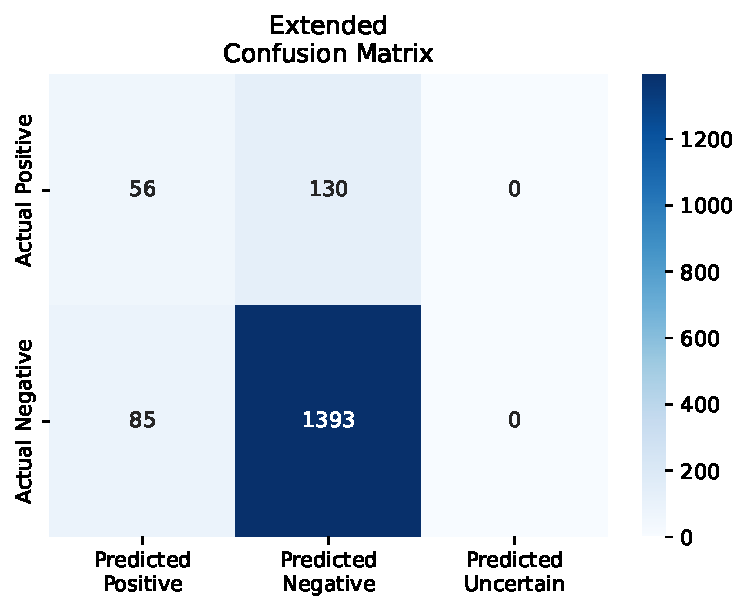
\includegraphics[width=\linewidth]{new_kdoqi_AVF.pdf}
        \caption{Baseline (KDOQI Guidelines)}
        \label{fig:vascular-access}
    \end{subfigure}
    \hfill
    \begin{subfigure}[b]{0.32\textwidth} % 確保寬度一致
        \centering
        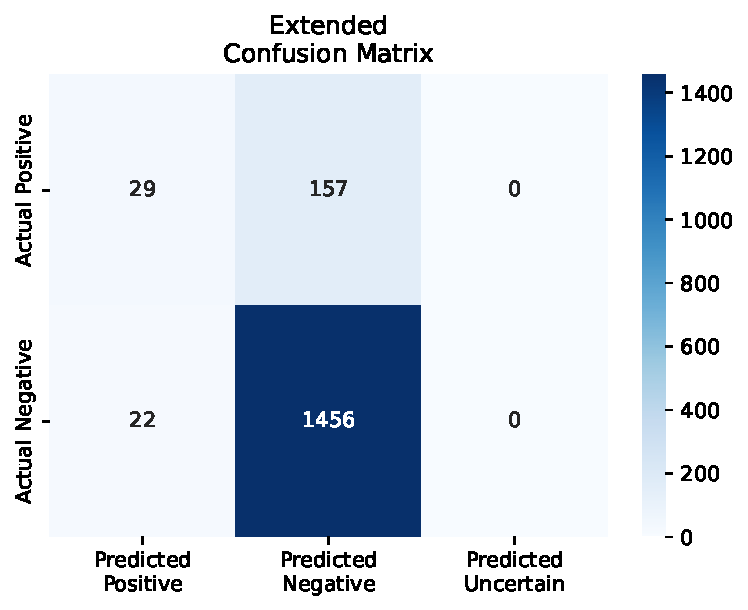
\includegraphics[width=\linewidth]{new_without_AVF.pdf}
        \caption{Our Method (Without Uncertain)}
        \label{fig:pta-symptom-method1}
    \end{subfigure}
    \hfill
    \begin{subfigure}[b]{0.32\textwidth}
        \centering
        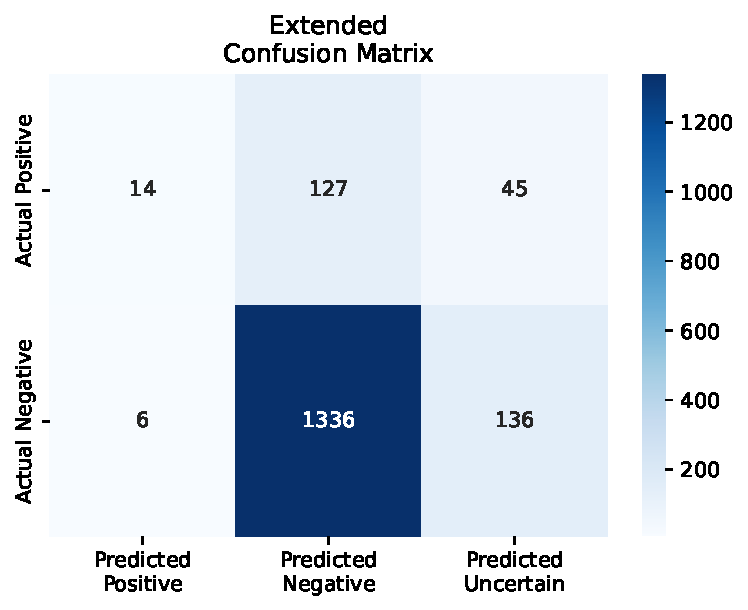
\includegraphics[width=\linewidth]{new_with_AVF.pdf}
        \caption{Our Method (With Uncertain)}
        \label{fig:pta-symptom-method2}
    \end{subfigure}

    \caption{AVF Dataset Extended Confusion Matrix}
    \label{fig:AVF_ECM}
\end{figure}

\begin{figure}[H]
    \centering
    % 第一行子圖
    \begin{subfigure}[b]{0.32\textwidth} % 設置子圖寬度為 1/3
        \centering
        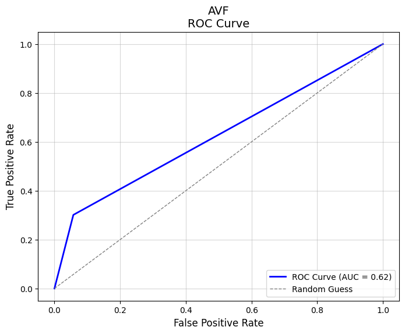
\includegraphics[width=\linewidth]{AVF_baseline_roc.png}
        \caption{Baseline (KDOQI Guidelines)}
        \label{fig:vascular-access-roc}
    \end{subfigure}
    \hfill % 添加水平間隔
    \begin{subfigure}[b]{0.32\textwidth}
        \centering
        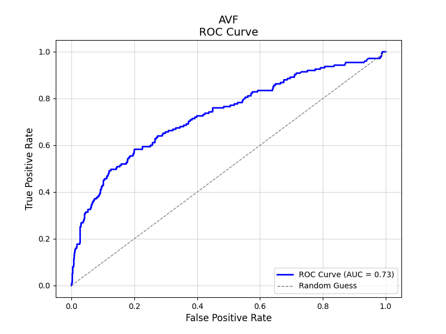
\includegraphics[width=\linewidth]{AVF_method1_roc.png}
        \caption{Our Method (Without Uncertain)}
        \label{fig:pta-symptom-method1-roc}
    \end{subfigure}
    \hfill
    \begin{subfigure}[b]{0.32\textwidth}
        \centering
        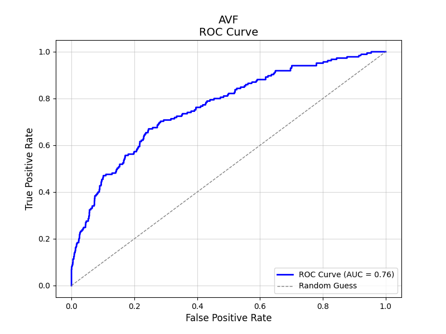
\includegraphics[width=\linewidth]{AVF_method2_roc.png}
        \caption{Our Method (With Uncertain)}
        \label{fig:pta-symptom-method2-roc}
    \end{subfigure}

    \caption{AVF Dataset ROC Curve Comparison}
    \label{fig:AVF_combined-roc}
\end{figure}

\begin{figure}[H]
    \centering
    % 第一行子圖
    \begin{subfigure}[b]{0.32\textwidth} % 調整每個子圖寬度為 1/3
        \centering
        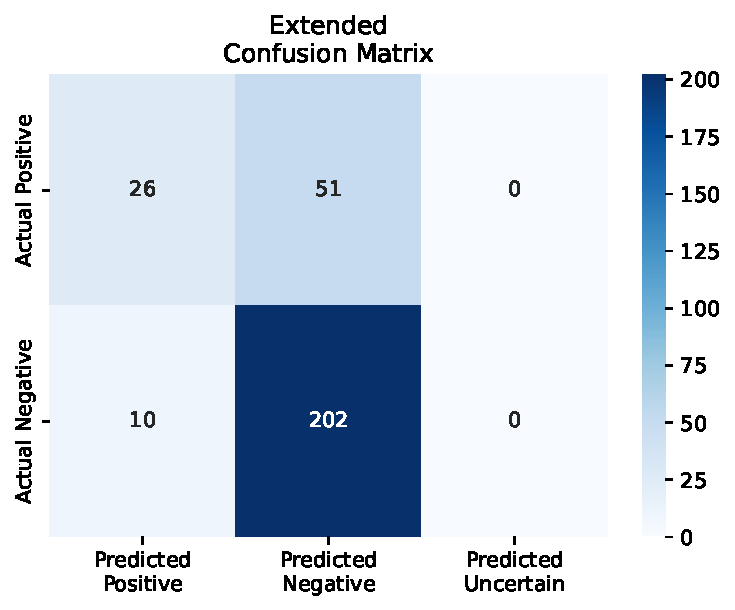
\includegraphics[width=\linewidth]{new_kdoqi_AVG.pdf}
        \caption{Baseline (KDOQI Guidelines)}
        \label{fig:vascular-access}
    \end{subfigure}
    \hfill % 水平間距
    \begin{subfigure}[b]{0.32\textwidth}
        \centering
        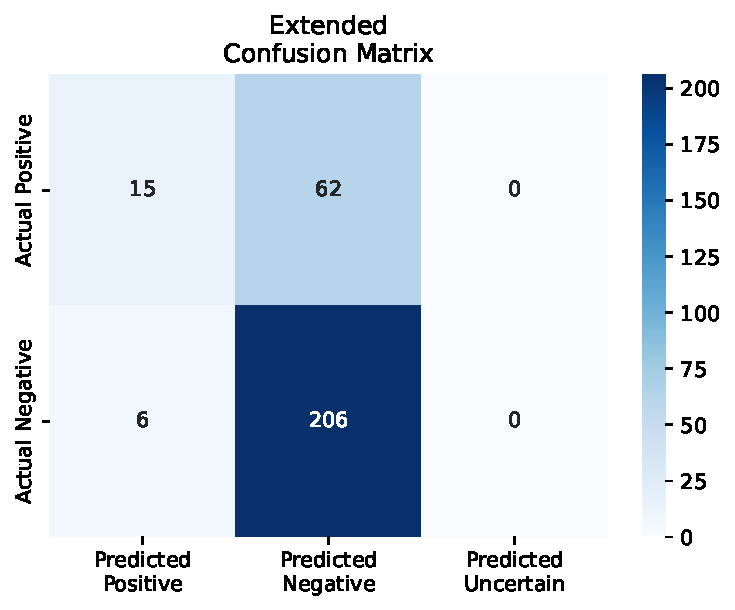
\includegraphics[width=\linewidth]{new_without_AVG.pdf}
        \caption{Our Method (Without Uncertain)}
        \label{fig:pta-symptom-method1}
    \end{subfigure}
    \hfill
    \begin{subfigure}[b]{0.32\textwidth}
        \centering
        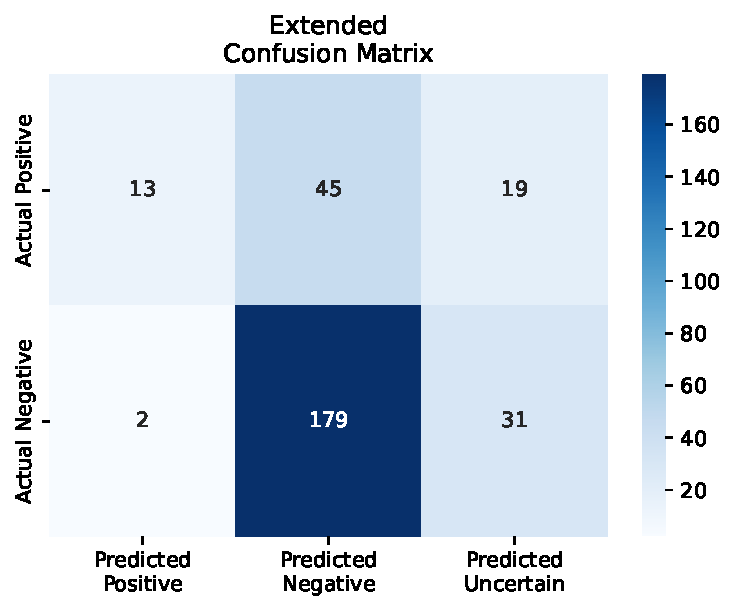
\includegraphics[width=\linewidth]{new_with_AVG.pdf}
        \caption{Our Method (With Uncertain)}
        \label{fig:pta-symptom-method2}
    \end{subfigure}

    \caption{AVG Dataset Extended Confusion Matrix}
    \label{fig:AVG_ECM}
\end{figure}

\begin{figure}[H]
    \centering
    % 調整每個子圖的寬度以適應頁面
    \begin{subfigure}[b]{0.32\textwidth} % 每張子圖寬度設置為頁面的 1/3
        \centering
        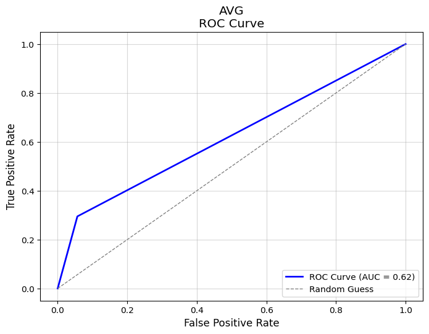
\includegraphics[width=\linewidth]{AVG_baseline_roc.png}
        \caption{Baseline (KDOQI Guidelines)}
        \label{fig:vascular-access-roc}
    \end{subfigure}
    \hfill % 水平間隔
    \begin{subfigure}[b]{0.32\textwidth}
        \centering
        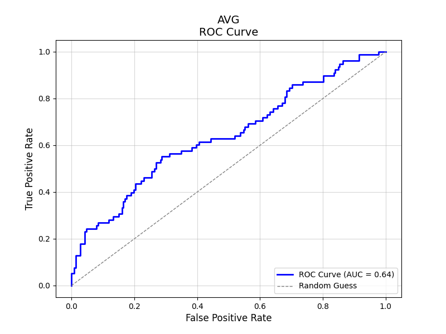
\includegraphics[width=\linewidth]{AVG_method1_roc.png}
        \caption{Our Method (Without Uncertain)}
        \label{fig:pta-symptom-method1-roc}
    \end{subfigure}
    \hfill
    \begin{subfigure}[b]{0.32\textwidth}
        \centering
        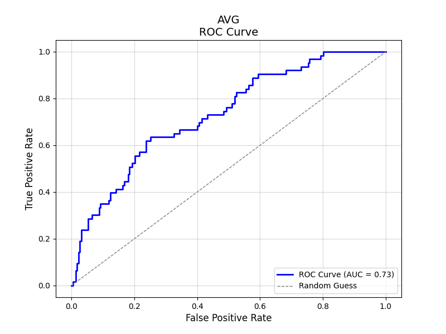
\includegraphics[width=\linewidth]{AVG_method2_roc.png}
        \caption{Our Method (With Uncertain)}
        \label{fig:pta-symptom-method2-roc}
    \end{subfigure}

    \caption{AVG Dataset ROC Curve Comparison}
    \label{fig:AVG_combined-roc}
\end{figure}

In comparison to the AVF dataset, the AVG dataset presents unique challenges due to its smaller size and higher surgical intervention rate. Despite these differences, the proposed uncertain-aware model consistently outperformed both the KDOQI guidelines and the model without uncertain classifications. The results emphasize the model’s adaptability and robustness, making it a valuable tool for supporting clinical decision-making in vascular access management.

\section{Conclusion}
\label{sec:guidelines}
Taiwan, with the highest global proportion of dialysis patients, faces challenges in managing vascular access dysfunction, a critical complication in hemodialysis. Early and accurate diagnosis is vital to mitigating risks and improving patient outcomes. This study introduces an uncertain-aware, tree-based machine learning framework to enhance diagnostic precision and address clinical data uncertainties.

The proposed methodology combines Multipass Uncertainty Estimation with Uncertain-Aware Data Classification, enabling robust predictions while accounting for ambiguous cases. An extended confusion matrix and novel metrics, such as leakage, overkill, and uncertainty, provide a comprehensive evaluation framework, emphasizing cautious and reliable decision-making.

Experimental results highlight the model's superior performance, with notable improvements in metrics like accuracy, AUC, and PPV across AVF and AVG datasets. The inclusion of uncertain classifications reduces error rates and enhances diagnostic reliability, outperforming traditional methods~\cite{Wu}.

By reallocating ambiguous predictions to an "Uncertain" category, the model ensures cautious decision-making, reducing misclassification risks. This approach aligns with clinical needs for reliable, interpretable, and actionable diagnostic tools, balancing precision and caution.

In summary, this study demonstrates the potential of integrating machine learning with indeterminacy analysis to improve clinical decision-making in complex datasets. The framework offers a scalable foundation for advancing medical AI, enabling more accurate diagnoses, reducing unnecessary interventions, and supporting timely treatment for dialysis patients.





\section*{Acknowledgment}

The authors acknowledge the use of Matplotlib for generating all plots and visualizations in this study. Additionally, GPT (Generative Pre-trained Transformer) from OpenAI was used to assist with language editing and formatting improvements. All scientific and technical content, including figures and analyses, was critically reviewed and verified by the authors to ensure accuracy and alignment with the study's context. The authors remain solely responsible for the integrity and conclusions of this work.


\begin{thebibliography}{1}

\bibitem{KDOQI} 
R. Navuluri and S. Regalado, ``The KDOQI 2006 Vascular Access Update and Fistula First Program Synopsis,'' \emph{Semin. Intervent. Radiol.}, vol. 26, no. 2, pp. 122--124, 2009, doi: 10.1055/s-0029-1222455.

\bibitem{Balch_2024} 
J. A. Balch, B. Shickel, A. Bihorac, G. R. Upchurch, and T. J. Loftus, ``Integration of AI in surgical decision support: improving clinical judgment,'' \emph{Global Surgical Education - J. Assoc. Surg. Educ.}, vol. 3, no. 1, p. 56, 2024, doi: 10.1007/s44186-024-00257-2.

\bibitem{Wu} 
C. K. Wu and C. H. Lin, ``Integrating vascular access surveillance with clinical monitoring for stenosis prediction,'' \emph{J. Nephrol.}, vol. 37, pp. 461--470, 2024, doi: 10.1007/s40620-023-01799-2.

\bibitem{decision_tree} 
L. Breiman, J. Friedman, R. A. Olshen, and C. J. Stone, \emph{Classification and Regression Trees}. 1st ed., Chapman and Hall/CRC, 1984, doi: 10.1201/9781315139470.

\bibitem{random_forest} 
L. Breiman, ``Random Forests,'' \emph{Machine Learning}, vol. 45, no. 1, pp. 5--32, 2001, doi: 10.1023/A:1010933404324.

\bibitem{XGBoost} 
T. Chen and C. Guestrin, ``XGBoost: A Scalable Tree Boosting System,'' \emph{arXiv preprint arXiv:1603.02754}, 2016.

\bibitem{LightGBM} 
G. Ke \emph{et al.}, ``LightGBM: A Highly Efficient Gradient Boosting Decision Tree,'' in \emph{Proc. NIPS}, 2017. [Online].

\bibitem{CatBoost} 
V. Dorogush, A. Ershov, and A. Gulin, ``CatBoost: Gradient Boosting with Categorical Features Support,'' \emph{arXiv preprint arXiv:1810.11363}, 2018.

\bibitem{Comparative_XGBoost} 
C. Bentéjac, A. Csörgő, and G. Martínez-Muñoz, ``A Comparative Analysis of XGBoost,'' \emph{arXiv preprint arXiv:1911.01914}, 2019.

\bibitem{9893798} 
I. D. Mienye and Y. Sun, ``A Survey of Ensemble Learning: Concepts, Algorithms, Applications, and Prospects,'' \emph{IEEE Access}, vol. 10, pp. 99129--99149, 2022, doi: 10.1109/ACCESS.2022.3207287.

\bibitem{Uncertainty_Quantification} 
V. Nemani \emph{et al.}, ``Uncertainty Quantification in Machine Learning for Engineering Design and Health Prognostics: A Tutorial,'' \emph{arXiv preprint arXiv:2305.04933}, 2023.

\bibitem{electronics11030396} 
M. Barandas \emph{et al.}, ``Uncertainty-Based Rejection in Machine Learning: Implications for Model Development and Interpretability,'' \emph{Electronics}, vol. 11, no. 3, p. 396, 2022, doi: 10.3390/electronics11030396.

\bibitem{perturbations} 
M. T. Ribeiro, S. Singh, and C. Guestrin, ``Why Should I Trust You?: Explaining the Predictions of Any Classifier,'' \emph{arXiv preprint arXiv:1602.04938}, 2016.

\bibitem{tree_based_model}
L. Grinsztajn, E. Oyallon, and G. Varoquaux, ``Why do tree-based models still outperform deep learning on tabular data?,'' \emph{arXiv preprint arXiv:2207.08815}, 2022.

\bibitem{Outperform_Boosted_Trees}
D. McElfresh, S. Khandagale, J. Valverde, V. Prasad C., G. Ramakrishnan, M. Goldblum, and C. White, ``When Do Neural Nets Outperform Boosted Trees on Tabular Data?,'' in \emph{Advances in Neural Information Processing Systems (NeurIPS) 2023}, vol. 36, pp. 76336--76369, Curran Associates, Inc., 2023.

\bibitem{Closer_Look}
H.-J. Ye, S.-Y. Liu, H.-R. Cai, Q.-L. Zhou, and D.-C. Zhan, ``A Closer Look at Deep Learning Methods on Tabular Datasets,'' \emph{arXiv preprint arXiv:2407.00956}, 2024.


\end{thebibliography}


\EOD

\end{document}
